\section{Theory}
	\subsection{Direct and Indirect Band Gap Semiconductors}
		Direct and indirect band gap semiconductors exhibit different energy momentum relationships between the valence band and conduction band. In direct band gap semiconductors, the valence band's top and conduction band's bottom occur at the same momentum ($k$) value within the band gap. On the other hand, in indirect band gap semiconductors, the maximum energy of the valence band and the minimum energy of the conduction band occur at different momentum ($k$) values. 
		\begin{figure}[H]
			\centering
			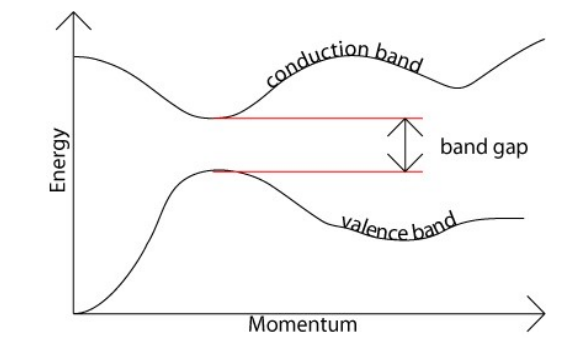
\includegraphics[width=0.8\columnwidth]{images/ut1.png}
			\caption{ Schematic of band structure for direct band gap material }
			\label{th:1}
		\end{figure}
		\begin{figure}[H]
			\centering
			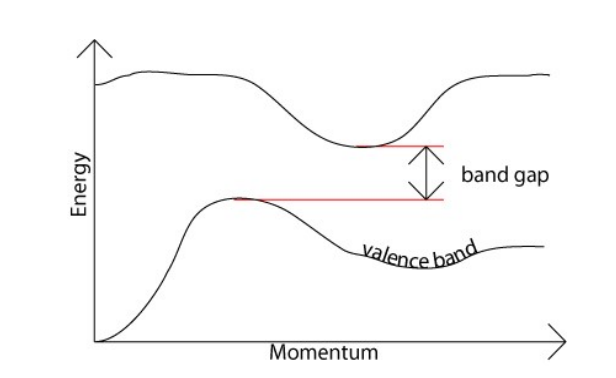
\includegraphics[width=0.8\columnwidth]{images/ut2.png}
			\caption{ Schematic of band structure for indirect band gap material }
			\label{th:2}
		\end{figure}

		In optical devices, the distinction between direct and indirect band gap semiconductors is particularly significant. The momentum of each photon is given by the formula $p = \sfrac{E}{c}$, where $c$ is the speed of light. With a speed of light value of $c = 3 \times 10^8 \, \text{m/s}$ and an energy on the order of $10^{-19} \, \text{J}$ for an optical photon, the momentum of a photon is typically very small.

		In direct band gap semiconductors, a photon with energy $E_g$ can easily produce an electron-hole pair, as the electron only needs a small amount of momentum. The energy of the photon is equal to the band gap energy ($E_g$). However, in indirect band gap semiconductors, the process of generating an electron-hole pair from an energy photon is more complex. The electron not only needs to absorb the energy from the photon, but also modify its momentum. This requires the electron to interact with a phonon, which is a type of lattice vibration.

		The interaction of three entities - an electron, a photon, and a phonon - makes the indirect process slower compared to the direct process. This same principle applies to the recombination of electrons and holes to generate photons. The recombination process is more efficient in direct band gap semiconductors, as it does not require phonon mediation, unlike in indirect band gap semiconductors.

		In a crystal lattice, only those phonons that conserve momentum participate in indirect transitions. This is why indirect band gap semiconductors, such as silicon, are not typically used in optical devices like LEDs and semiconductor lasers. In contrast, direct band gap semiconductors like gallium arsenide are commonly employed for these applications, as they allow for more efficient photon generation and recombination.




	\subsection{UV-vis Spectroscopy for Optical Band Gap Measurement:}
		UV-vis spectroscopy is a technique used to determine the optical band gap of semiconductor materials. It measures the absorption of light as a function of wavelength, providing information on the electronic transitions that occur within the material. The optical band gap is closely related to the electronic band gap, which is defined as the energy difference between the conduction band maximum and the valence band lowest.
		
		The Beer-Lambert law, given by Equation \ref{eq:beer-lambert}, relates the absorbance ($A$) of a sample to the molar absorptivity coefficient ($\epsilon$), the concentration of the absorbing species ($c$), and the path length of light through the sample ($l$). Absorbance is calculated as the negative logarithm of the ratio of transmitted intensity ($I_T$) to incident intensity ($I_O$).
		
		\begin{equation}
			\label{eq:beer-lambert}
			A=\epsilon c l=-\log_{10}\left(\frac{I_T}{I_O}\right)
		\end{equation}
		
		The absorption coefficient ($\alpha$) of the material, which represents the extent to which the material absorbs light, is calculated using Equation \ref{eq:absorption-coefficient}. It is determined from the absorbance ($A$) and the path length of light ($l$) through the sample.
		
		\begin{equation}
			\label{eq:absorption-coefficient}
			\alpha (\text{cm}^{-1})= \frac{\ln(10) \times A}{l(\text{cm})}
		\end{equation}
		
		The Tauc method, as given by Equation \ref{eq:tauc-method}, is commonly used to determine the energy band gap ($E_g$) of a material. It relates the absorption coefficient ($\alpha$) to the incident photon energy ($h\nu$), where $h$ is the Planck's constant and $\nu$ is the frequency of the incident light. The parameter $n$ in Equation \ref{eq:tauc-method} depends on the type of transition. For direct allowed transitions, $n=\sfrac{1}{2}$, and for indirect allowed transitions, $n=2$.
		
		\begin{equation}
			\label{eq:tauc-method}
			\alpha(h\nu) = A(h\nu-E_g)^n
		\end{equation}
		
		Equation \ref{eq:direct-band-gap} represents the relationship between the absorption coefficient ($\alpha$) and the incident photon energy ($h\nu$) for direct band gap materials, where the band gap energy ($E_g$) is raised to the power of 0.5.
		
		\begin{equation}
			\label{eq:direct-band-gap}
			\alpha(h\nu) = A(h\nu-E_g)^{0.5}
		\end{equation}
		
		Equation \ref{eq:indirect-band-gap} represents the relationship between the absorption coefficient ($\alpha$) and the incident photon energy ($h\nu$) for indirect band gap materials, where the band gap energy ($E_g$) is modified by the additional energy of a phonon ($E_p$) emitted or absorbed during the transition. The sign `+' corresponds to phonon emission, and the sign `-' corresponds to phonon absorption.
		
		\begin{equation}
			\label{eq:indirect-band-gap}
			\alpha(h\nu) = A(h\nu-E_g\pm E_p)^n
		\end{equation}
